%% -*- coding:utf-8 -*-
%%%%%%%%%%%%%%%%%%%%%%%%%%%%%%%%%%%%%%%%%%%%%%%%%%%%%%%%%
%%   $RCSfile: 2-hpsg-formalismus.tex,v $
%%  $Revision: 1.17 $
%%      $Date: 2008/09/30 09:14:41 $
%%     Author: Stefan Mueller (CL Uni-Bremen)
%%    Purpose: 
%%   Language: LaTeX
%%%%%%%%%%%%%%%%%%%%%%%%%%%%%%%%%%%%%%%%%%%%%%%%%%%%%%%%%





\ifthenelse{\boolean{hpsg-buch}}{
\chapter{Der Formalismus}
\label{kap-merkmalstrukturen}

In diesem Kapitel werden Merkmalstrukturen eingeführt, mit deren Hilfe
wir alle linguistischen Objekte modellieren werden.
}{% GT-Buch
\chapter{Merkmalbeschreibungen}
\label{Kap-Merkmalbeschreibungen}

Im vorigen Kapitel war schon die Rede von Mengen von Merkmal"=Wert"=Paaren, die linguistische
Objekte beschreiben. In diesem Kapitel werden Merkmalstrukturen bzw.\ Merkmalbeschreibungen
eingeführt, die in Theorien wie LFG, HPSG, Konstruktionsgrammatik und auch in Varianten von
Kategorialgrammatik und TAG eine Rolle spielen. Diese Kapitel stellt somit die Grundlagen für die
folgenden Kapitel dar.

}
Für Merkmalstrukturen finden sich auch folgende Bezeichnungen: 
\begin{itemize}
\item Merkmal-Wert-Struktur\is{Merkmal"=Wert"=Struktur}
\item Attribut-Wert-Struktur\is{Attribut"=Wert"=Struktur}
\item \emph{feature structure}
\end{itemize}
Merkmalstrukturen sind komplexe Gebilde, die alle Eigenschaften eines linguistischen
Objekts modellieren. Der Linguist arbeitet meist mit Merkmalbeschreibungen, die nur Ausschnitte der
Merkmalstruktur beschreiben. Der Unterschied zwischen Modell und Beschreibung wird im Abschnitt~\ref{sec-modelle-theorien}
noch genauer erklärt. Andere Bezeichnungen für Merkmalbeschreibungen sind:
\begin{itemize}
\item \emph{attribute-value matrix} (AVM)
\item \emph{feature matrix}
\end{itemize}
Ich beschränke mich im folgenden auf das unbedingt Nötige, um den formalen Teil
des Buches so klein wie möglich zu halten. Der interessierte Leser sei auf
\citet{Shieber86a}, \citet[Kapitel~2]{ps}, \citet{Johnson88}, \citet{Carpenter92a},
\citet{King94a} und \citet{Richter2004a-u} verwiesen. Shiebers Buch ist
eine leicht lesbare Einführung in Unifikationsgrammatiken, Kings und Richters Arbeiten, die wichtige Grundlagen
für die HPSG darstellen, dürften mathematischen Laien unzugänglich bleiben.
Wichtig ist, dass es diese Arbeiten gibt und dass man weiß, dass die Theorie
auf einem sicheren Fundament steht.

\section{Merkmalbeschreibungen}

Wenn\is{Merkmalbeschreibung|(} wir sprachliche Zeichen beschreiben wollen, wollen wir etwas über ihre Eigenschaften
aussagen. Wir können \zb einem Nomen Kasus, Genus, Numerus und Person zuordnen. Für das
Wort \emph{Mannes} müßten diese Merkmale die Werte \emph{Genitiv}, \emph{maskulin}, \emph{Singular} und \emph{3} haben.
Schreibt man dies als Liste von Merkmal"=Wert"=Paaren auf, so hat man bereits eine Merkmalbeschreibung:
\ea
Merkmal"=Wert"=Paare für \emph{Mannes}:\\
\ms{
kasus   & Genitiv\\
genus   & maskulin\\
numerus & Singular\\
person  & 3\\
}
\z
Mit Merkmalbeschreibungen kann man natürlich ganz verschiedene Dinge beschreiben. Zum Beispiel kann
man mit (\mex{1}) einen Menschen beschreiben:
\ea
\ms{
vorname    & max\\
nachname   & meier\\
geburtstag & 10.10.1985\\
}
\z
Menschen sind mit anderen Menschen verwandt, was man ebenfalls in Merkmal"=Wert"=Paaren
ausdrücken kann. So kann man \zb die Tatsache, dass Max Meier einen Vater namens Peter
Meier hat, repräsentieren, indem man (\mex{0}) wie folgt erweitert:
\ea
\ms{
vorname    & max\\
nachname   & meier\\
geburtstag & 10.10.1985\\
vater      & \ms{
             vorname & peter\\
             nachname  & meier\\
             geburtstag   & 10.05.1960\\
             vater     & \ldots\\
             mutter     & \ldots\\
             }\\
mutter     & \ldots\\
}
\z
Der Wert des \textsc{vater}"=Merkmals ist dann eine Merkmalbeschreibung, die dieselben Merkmale
wie (\mex{-1}) hat.

Ein \emph{Pfad}\is{Pfad} in einer Merkmalbeschreibung ist eine Folge von Merkmalen, 
die in der Merkmalbeschreibung unmittelbar aufeinander folgen.
Der \emph{Wert eines Pfades} ist die Merkmalbeschreibung am Ende des Pfades. So ist
der Wert von \textsc{vater$|$geburtstag} das Datum \emph{10.05.1960}.

Es fallen einem sofort mehrere Merkmale ein, die man noch in Repräsentationen wie (\mex{0})
aufnehmen könnte. Man überlege sich, wie Information über Töchter oder Söhne in 
(\mex{0}) integriert werden kann.

Eine naheliegende Lösung ist, weitere Merkmale für \textsc{tochter} und \textsc{sohn}
einzuführen:
\ea
\ms{
vorname    & max\\
nachname   & meier\\
geburtstag & 10.10.1985\\
vater      & \ldots\\
mutter     & \ldots\\
tochter    & \ldots\\   
}
\z
Diese Lösung ist jedoch nicht befriedigend, da sie es nicht ohne weiteres
ermöglicht, Menschen mit mehreren Töchtern zu beschreiben. Sollte man dann
Merkmale wie \textsc{tochter-1} oder \textsc{tochter-3} einführen?
\ea
\ms{
vorname    & max\\
nachname   & meier\\
geburtstag & 10.10.1985\\
vater      & \ldots\\
mutter     & \ldots\\
tochter-1  & \ldots\\
tochter-2  & \ldots\\
tochter-3  & \ldots\\
}
\z
Wieviele Merkmale will man annehmen? Wo ist die Grenze?
Was ist der Wert von \textsc{tochter"=32}?

Geschickter ist es hier, eine Liste\is{Liste} zu verwenden. Listen werden mit spitzen
Klammern dargestellt. Zwischen den spitzen Klammern können beliebig
viele Elemente stehen. Ein Spezialfall ist, dass kein Element zwischen den
Klammern steht, man spricht dann von \emph{der leeren Liste}. Im folgenden Beispiel
hat Max Meier eine Tochter namens Clara, die selbst keine Töchter hat:
\ea
\ms{
vorname    & max\\
nachname   & meier\\
geburtstag & 10.10.1985\\
vater      & \ldots\\
mutter     & \ldots\\
töchter    & \liste{ \ms{
                     vorname    & clara\\
                     nachname   & meier\\
                     geburtstag & 10.10.2004\\
                     vater      & \ldots\\
                     mutter     & \ldots\\
                     töchter    & \liste{ }\\   
} }\\   
}
\z
Nun stellt sich die Frage: Was ist mit Söhnen? Soll man eine Liste der Söhne einführen?
Wollen wir zwischen Söhnen und Töchtern differenzieren? 
Sicher ist das Geschlecht der Kinder eine wichtige Eigenschaft, aber es ist eine Eigenschaft
der beschriebenen Objekte. Alle Menschen haben ein Geschlecht. Die Beschreibung in (\mex{1})
ist also eine adäquatere Repräsentation:

\ea
\ms{
vorname    & max\\
nachname   & meier\\
geburtstag & 10.10.1985\\
\textbf{\textsc{geschlecht}} & \emph{\textbf{männlich}}\\
vater      & \ldots\\
mutter     & \ldots\\
\emph\textsc{kinder}     & \liste{ \ms{
                     vorname    & clara\\
                     nachname   & meier\\
                     geburtstag & 10.10.2004\\
                     \textbf{\textsc{geschlecht}} & \emph{\textbf{weiblich}}\\
                     vater      & \ldots\\
                     mutter     & \ldots\\
                     kinder     & \liste{ }\\   
} }\\   
}
\z
Nun kann man fragen, warum die Eltern nicht auch in einer Liste repräsentiert werden.
In der Tat wird man ähnliche Fragen auch in linguistischen Aufsätzen wiederfinden:
Wie wird Information am zweckmäßigsten organisiert? Für eine Repräsentation der Beschreibungen
der Eltern unter separaten Merkmalen spricht eventuell, dass man bestimmte Aussagen über die
Mutter bzw.\ den Vater machen möchte, ohne erst ein passendes Element aus einer Liste suchen
zu müssen.

Wenn die Reihenfolge der Elemente egal ist, verwendet man statt Listen auch Mengen\is{Menge}.
Mengen werden mit geschweiften Klammern geschrieben.\footnote{
 Die Beschreibung von Mengen ist technisch aufwendig.
 Wir würden in diesem Buch Mengen nur zum Aufsammeln von semantischer Information verwenden.
 Dies kann genauso gut mit Hilfe von Listen gemacht werden, weshalb wir hier auf die
 Einführung der Mengen verzichten und statt der Mengen Listen verwenden.%
}

\section{Typen}
\label{sec-formalismus-typen}

Im\is{Typ|(} vorigen Abschnitt wurden aus Merkmal"=Wert"=Paaren bestehende
Merkmalbeschreibungen vorgestellt, und es wurde gezeigt, dass es sinnvoll ist,
komplexe Werte für Merkmale zuzulassen.  In diesem Abschnitt werden die
Merkmalbeschreibungen um Typen erweitert. Merkmalbeschreibungen, denen ein Typ
zugeordnet wurde, werden auch \emph{typisierte Merkmalbeschreibungen} genannt.
Typen sagen etwas darüber aus, welche Merkmale zu einer
bestimmten Struktur gehören müssen bzw.\ zu einer Beschreibung der
Struktur gehören dürfen. Die bisher diskutierte Beschreibung beschreibt
Objekte vom Typ \type{person}.
\ea
\ms[person]{
vorname    & max\\
nachname   & meier\\
geburtstag & 10.10.1985\\
geschlecht & männlich\\
vater      & \ldots\\
mutter     & \ldots\\
kinder     & \liste{ \ldots, \ldots }\\   
}
\z
Der Typ wird \textit{kursiv} gesetzt. 

In einer Typspezifikation wird festgelegt, welche Eigenschaften ein modelliertes
Objekt hat. In der Theorie kann man dann nur über diese Eigenschaften sinnvoll etwas
aussagen. Eigenschaften wie \textsc{Betriebsspannung} sind für Objekte vom
Typ \textit{person} nicht relevant. Wenn man den Typ eines beschriebenen Objekts kennt,
weiß man also, dass das Objekt bestimmte Eigenschaften haben muss, auch wenn man
die genauen Werte (noch) nicht kennt. So ist (\mex{1}) eine Beschreibung von
Max Meier, obwohl sie \zb keine Information über Max' Geburtstag enthält:
\ea
\ms[person]{
vorname    & max\\
nachname   & meier\\
geschlecht & männlich\\
}
\z
Man weiß aber, dass Max Meier an irgendeinem Tag Geburtstag haben muss, da die
Beschreibung vom Typ \textit{person} ist. Die Frage \emph{Wann hat Max Geburtstag?}
ist also in bezug auf eine von (\mex{0}) beschriebene Struktur sinnvoll, was für die Frage
\emph{Welche Betriebsspannung hat Max?} nicht der Fall ist. Wenn wir wissen, dass ein Objekt vom Typ
\textit{person} ist, haben wir sozusagen seine Grobstruktur:
\ea
\ms[person]{
vorname    & vorname\\
nachname   & nachname\\
geburtstag & datum\\
geschlecht & geschlecht\\
vater      & person\\
mutter     & person\\
kinder     & list of person\\   
}
\z
In (\mex{0}) und (\mex{-1}) sind auch Werte von Merkmalen wie \textsc{vorname} kursiv gesetzt. Diese Werte sind auch
Typen. Sie unterscheiden sich jedoch von Typen wie \type{person} dadurch, dass zu ihnen keine
Merkmale gehören. Solche Typen werden \emph{atomar}\is{Typ!atomarer} genannt.

Typen sind in Hierarchien\is{Typhierarchie|(} organisiert.
%% \footnote{
%%   Auf das Verhältnis von Typen in Hierarchien zueinander werde ich in Kapitel~\ref{sec-typen} noch genauer eingehen.%
%% }
Man kann \zb die Untertypen \textit{frau} und \textit{mann} für \textit{person}
definieren. Diese würden sich dann durch die Festlegung des Geschlechts auszeichnen.
(\mex{1}) zeigt eine Merkmalbeschreibung des Typs \textit{frau}. Die für \textit{mann}
wäre analog.
\ea
\ms[frau]{
vorname    & vorname\\
nachname   & nachname\\
geburtstag & datum\\
geschlecht & weiblich\\
vater      & mann\\
mutter     & frau\\
kinder     & list of person\\   
}
\z
Man kann sich hier jetzt wieder fragen, ob man das Merkmal \textsc{geschlecht} überhaupt
noch braucht. Die notwendige Information ist ja bereits im Typ \type{frau} repräsentiert.
Die Frage, ob man bestimmte Information als Wert eines speziellen Merkmals repräsentiert oder die
Information in einem Typ ohne ein entsprechendes eigenständiges Merkmal unterbringt,  
wird auch bei der Arbeit an linguistischen Analysen wieder auf"|tauchen.
Die beiden Alternativen unterscheiden sich vor allem darin, dass Information, die
über Typen modelliert wird, für die im Abschnitt~\ref{sec-strukturteilung} besprochenen Strukturteilungen
nicht ohne weiteres %###### FR: geht wohl doch, gibt Beweis von Gerald
zugänglich ist.

%% Als Beispiel sei hier die Typhierarchie
%% unter dem Typ für die Wortart (\emph{part of speech}) diskutiert, die Abbildung~\vref{fig-untertypen-pos}
%% zeigt.
%% \begin{figure}[htbp]
%% \centerline{\begin{tabular}{ccccccc}
%% \multicolumn{6}{c}{\rnode{p-o-s}\textit{p-o-s}}\\[4ex]
%% \rnode{adj}\textit{adj} & \rnode{adv}\textit{adv} & \rnode{det}\textit{det} & \rnode{noun}\textit{noun} & \rnode{prep}\textit{prep} & \rnode{verb}\textit{verb}\\
%% \end{tabular}
%% \ncline{p-o-s}{adj}\ncline{p-o-s}{adv}\ncline{p-o-s}{det}\ncline{p-o-s}{noun}\ncline{p-o-s}{prep}\ncline{p-o-s}{verb}}%
%% \caption{\label{fig-untertypen-pos}Eine Beispiel"=Typhierarchie für die Typen unter \emph{part of speech}}
%% \end{figure}
%% Der Typ \textit{p-o-s} ist der allgemeinste Typ. Alle Wörter haben eine Wortart,
%% die einem Untertyp von \textit{p-o-s} entspricht, also \zb Adjektiv \textit{adj} oder Präposition \textit{prep}.
%% Auf das Verhältnis von Typen in Hierarchien zueinander werde ich in Kapitel~\ref{sec-typen} noch genauer eingehen.

Typhierarchien spielen eine wichtige Rolle für das Erfassen linguistischer
Generalisierungen, weshalb im folgenden Typhierarchien und die Vererbung\is{Vererbung}
von Beschränkungen und Information an einem weiteren Beispiel erklärt werden sollen.
Typhierarchien kann man sich wie eine effektive Organisation von Wissen vorstellen.
In einem Nachschlagewerk sind die einzelnen Einträge miteinander verknüpft, so steht beim Eintrag für Affe
und für Maus jeweils ein Zeiger auf Säugetier. Die Beschreibung, die bei Säugetier
steht, muss somit bei den Einträgen für untergeordnete Konzepte nicht wiederholt werden.
Genauso könnte man, wenn man verschiedene elektrische Geräte beschreiben will,
die Hierarchie in Abbildung~\vref{fig-elektr-geraet} verwenden.
\begin{figure}
% \centerline{\begin{tabular}{cccc}
% \multicolumn{4}{c}{\rnode{ed}{\textit{elektrisches Gerät}}}\\[6ex]
% \rnode{p}{\textit{druckendes Gerät}} & & \rnode{sc}{\textit{scannendes Gerät}} & \rnode{other}{\rule[-0.5ex]{0cm}{2.5ex}\ldots}\\[6ex]
% \rnode{printer}{\textit{Drucker}}   & \rnode{copy}{\textit{Kopierer}}  & \rnode{scanner}{\textit{Scanner}}\\[6ex]
% \rnode{l-p}{\textit{Laserdrucker}}  & \rnode{other-p}{\rule[-0.5ex]{0cm}{2.5ex}\ldots}  & \rnode{negscan}{\textit{Negativscanner}} & \rnode{other-sc}{\rule[-0.5ex]{0cm}{2.5ex}\ldots}\\
% \end{tabular}}
% \ncline{ed}{p}\ncline{ed}{sc}\ncline{ed}{other}%
% \ncline{p}{copy}\ncline{p}{printer}\ncline{printer}{l-p}\ncline{printer}{other-p}%
% \ncline{sc}{copy}%
% \ncline{sc}{scanner}\ncline{scanner}{negscan}\ncline{scanner}{other-sc}%
\centerline{%
\begin{forest} 
type hierarchy
[elektrisches Gerät, calign=midpoint, calign children={1}{2},
  [durckendes Gerät,calign=first
    [Drucker,calign=first
      [Laser-Drucke]
      [\ldots]]
    [Kopierer]]
  [scannendes Gerät,calign=last
    [,identify=!r12]
    [Scanner,calign=first
      [Negativ-Scanner]
      [\ldots]]]
  [\ldots]]
\end{forest}}

\caption{\label{fig-elektr-geraet}Nicht"=linguistisches Beispiel für Mehrfachvererbung}
\end{figure}
Der allgemeinste Typ \textit{elektrisches Gerät} steht in Abbildung~\ref{fig-elektr-geraet} ganz oben.
Elektrische Geräte haben bestimmte Eigenschaften, \zb eine Stromversorgung mit einer bestimmten
Leistungsaufnahme. Alle Untertypen von \textit{elektrisches Gerät} "`erben"' diese Eigenschaft. So haben
\zb \textit{druckendes Gerät} und \textit{scannendes Gerät} ebenfalls eine Stromversorgung mit einer
bestimmten Leistungsaufnahme. Ein \textit{druckendes Gerät} kann Information ausgeben, und ein \textit{scannendes Gerät}
kann Information einlesen. Ein \textit{Kopierer} kann sowohl Information einlesen als auch ausgeben.
Kopierer haben sowohl Eigenschaften einlesender Geräte als auch Eigenschaften druckender Geräte. Das wird
durch die beiden Verbindungen zu den Obertypen in Abbildung~\ref{fig-elektr-geraet} ausgedrückt.
Ist ein Typ gleichzeitig Untertyp mehrerer Obertypen, so spricht man auch von \emph{Mehrfachvererbung}\is{Vererbung!Mehrfach-}
(\emph{multiple inheritance}). Können Geräte nur drucken, aber nicht scannen, so sind sie vom Typ
\emph{Drucker}. Dieser Typ hat dann wieder spezifischere Untertypen, die bestimmte besondere Eigenschaften
haben, \zb \textit{Laserdrucker}. Bei den Untertypen können neue Merkmale hinzukommen, es kann aber
auch sein, dass Werte für bereits existierende Merkmale spezifischer werden. So ist \zb beim
Typ \textit{Negativscanner} im Vergleich zu seinem Supertyp \textit{Scanner} 
die Art des Eingabematerials sehr eingeschränkt. 

Die Objekte, die man modelliert, haben immer einen maximal spezifischen Typ. In unserem Beispiel
bedeutet das, dass wir Objekte vom Typ \type{Laserdrucker} und \type{Negativscanner} haben können aber nicht
vom Typ \type{druckendes Gerät}. Das liegt daran, dass \type{druckendes Gerät} nicht maximal
spezifisch ist, denn dieser Typ hat Untertypen.

Typhierarchien mit Mehrfachvererbung sind ein wichtiges Mittel, um linguistische Generalisierungen
auszudrücken. Typen für Wörter oder Phrasen, die in diesen Hierarchien ganz oben stehen, entsprechen
Beschränkungen über linguistischen Objekten, die für alle linguistischen Objekte in allen Sprachen
Gültigkeit haben. Untertypen dieser allgemeinen Typen können sprachklassen- oder sprachspezifisch sein.%
\is{Typ|)}\is{Typhierarchie|)}

\section{Disjunktion}

Disjunktionen\is{Disjunktion|(} kann man verwenden, wenn man ausdrücken möchte, dass ein bestimmtes Objekt
verschiedene Eigenschaften haben kann. Wenn wir \zb zwanzig Jahre nach dem Verlassen der Schule
ein Klassentreffen organisieren wollen und uns nicht mehr genau an die Namen der Klassenkameraden erinnern,
dann könnte man im World Wide Web nach "`Julia (Warbanow oder Barbanow)"' suchen.
In Merkmalbeschreibungen wird das Oder durch `$\vee$'\is{$\vee$} ausgedrückt.
\ea
\ms[person]{
 vorname  & Julia\\
 nachname & Warbanow $\vee$ Barbanow\\
}
\z
Manche Internetsuchmaschinen lassen durch `oder' verknüpfte Anfragen nicht zu. Man muss
dann zwei einzelne Anfragen nämlich nach "`Julia Warbanow"' und nach "`Julia Barbanow"'
stellen. Das entspricht den beiden folgenden, disjunktiv verknüpften Beschreibungen:
\ea
\ms[person]{
 vorname  & Julia\\
 nachname & Warbanow\\
} $\vee $
\ms[person]{
 vorname  & Julia\\
 nachname & Barbanow\\
}
\z
Da wir Typhierarchien als Ausdrucksmittel zur Verfügung haben, können wir manchmal auf die
disjunktive Spezifikation von Werten verzichten und statt dessen den Obertyp\is{Typ} angeben:
Für \type{Drucker} $\vee$ \type{Kopierer} kann man auch \type{druckendes Gerät} schreiben,
wenn man die Typhierarchie in Abbildung~\vref{fig-elektr-geraet} zugrundelegt.%
\is{Disjunktion|)}

\section{Strukturteilung}
\label{sec-strukturteilung}

Strukturteilung\is{Strukturteilung|(} ist ein wichtiger Bestandteil des HPSG"=Formalismus. Sie dient
dazu auszudrücken, dass gewisse Teile einer Struktur identisch sind. Ein linguistisches
Beispiel für eine Identität von Werten ist die Kongruenz\is{Kongruenz}. In Sätzen wie denen in (\mex{1})
muss der Numerus"=Wert der Nominalphrase mit dem des Verbs identisch sein:
\eal
\ex[]{
Der Mann schläft.
}
\ex[]{
Die Männer schlafen.
}
\ex[*]{
Der Mann schlafen.
}
\zl
Die Identität von Werten wird durch Boxen mit Zahlen darin verdeutlicht.
Die Boxen kann man auch als Variablen auf"|fassen.

Man kann bei der Beschreibung von Objekten zwischen Gleichheit und Identität
unterscheiden. Eine Aussage über die Identität von Werten ist stärker. Als
Beispiel soll die folgende Merkmalbeschreibung dienen, die Information
über die Kinder enthält, die Max' Vater bzw.\ Max' Mutter hat:
\ea
\ms[person]{
vorname    & max\\
nachname   & meier\\
geburtstag & 10.10.1985\\
vater      & \ms[person]{
              vorname  & peter\\
              nachname & meier\\
              kinder   & \liste{ \ms[person]{
                                 vorname & klaus\\
                                 }, \ldots }\\
             }\\
mutter     & \ms[person]{
              vorname  & anna\\
              nachname & meier\\
              kinder   & \liste{ \ms[person]{
                                 vorname & klaus\\
                                 }, \ldots }\\
             }\\
}
\z
Unter den Pfaden \textsc{vater$|$kinder} und \textsc{mutter$|$kinder} steht jeweils
eine Liste mit einer Beschreibung für eine Person mit dem Vornamen Klaus.
Die Frage, ob die Merkmalbeschreibung ein Kind oder zwei Kinder von Peter und Anna
beschreibt, kann nicht geklärt werden. Es ist durchaus möglich,
dass es sich um zwei Kinder aus früheren Verbindungen handelt, die zufällig
beide Klaus heißen.

Mit Hilfe von Strukturteilung kann man die Identität der beiden Werte
festmachen:
\ea
\ms[person]{
vorname    & max\\
nachname   & meier\\
geburtstag & 10.10.1985\\
vater      & \ms[person]{
              vorname  & peter\\
              nachname & meier\\
              kinder   & \liste{ \ibox{1} \ms[person]{
                                 vorname & klaus\\
                                 }, \ldots }\\
             }\\
mutter     & \ms[person]{
              vorname  & anna\\
              nachname & meier\\
              kinder   & \liste{ \ibox{1}, \ldots }\\
             }\\
}
\z
In (\mex{0}) ist Klaus ein Kind, das beide gemeinsam haben. Alles, was innerhalb der Klammer unmittelbar
nach \iboxt{1} steht, ist an beiden Stellen genauso vorhanden. Man kann sich die \iboxt{1}
als einen Zeiger bzw.\ Verweis auf eine % normalerweise (kann auch Teilaspekte verteilt angeben)
nur einmal beschriebene Struktur
vorstellen. Eine Frage ist noch offen: Was ist mit Max? Max ist ja auch ein
Kind seiner Eltern und sollte demnach auch in der Liste der Kinder seiner
Eltern auf"|tauchen. In (\mex{0}) gibt es an zwei Stellen drei Punkte. Diese Auslassungszeichen stehen für Aussagen
über die weiteren Kinder von Peter und Anna Meier. Unser Weltwissen sagt uns, dass die beiden jeweils mindestens
noch ein Kind haben müssen, nämlich Max Meier selbst. Im folgenden Abschnitt wird gezeigt, wie
man das formal ausdrücken kann.%
\is{Strukturteilung|)}


\section{Zyklische Strukturen}


Wir\is{Zyklus|(} haben die Strukturteilung eingeführt, damit wir sagen können, dass
Max' Eltern einen gemeinsamen Sohn Klaus haben. Es wäre nicht adäquat,
Max jeweils separat in die Kinder"=Listen seiner Eltern aufzunehmen.
Wir müssen erfassen, dass jeweils derselbe Max in den Kinder"=Listen
steht, und außerdem muss auch noch sichergestellt werden, dass das
Objekt, das als Kind beschrieben wird, mit dem Gesamtobjekt identisch
ist, denn sonst hätten wir wieder die Situation, in der Max' Eltern
noch ein zweites Kind namens Max haben könnten.
Die Beschreibung in (\mex{1})\vpageref{bsp-avm-zyklen} erfaßt die Zusammenhänge korrekt.
\begin{figure}[htbp]
\ea
\label{bsp-avm-zyklen}
\ibox{2} \ms[person]{
vorname    & max\\
nachname   & meier\\
geburtstag & 10.10.1985\\
vater      & \ms[person]{
              vorname  & peter\\
              nachname & meier\\
              kinder   & \liste{ \ibox{1} \ms[person]{
                                 vorname & klaus\\
                                 }, \ibox{2} }\\
             }\\
mutter     & \ms[person]{
              vorname  & anna\\
              nachname & meier\\
              kinder   & \liste{ \ibox{1}, \ibox{2} }\\
             }\\
}
\z
\vspace{-\baselineskip}\end{figure}
Strukturen, die durch Beschreibungen wie (\mex{0}) beschrieben werden, werden zyklisch genannt, weil man, wenn man bestimmten
Pfaden folgt, im Kreis gehen kann: \ZB den Pfad \textsc{vater$|$""kinder$|$""\ldots$|$""vater$|$""kinder$|$\ldots}\footnote{
  Die Punkte stehen hierbei für den Pfad zu \iboxt{2} in der Liste, die
  Wert von \textsc{kinder} ist. Siehe Übungsaufgabe~\ref{ua-liste}.%
}
kann man unendlich lange wiederholen.
\is{Zyklus|)}

\section{Unifikation}
\label{sec-unifikation}

\mbox{}\is{Unifikation|(}%
Grammatikregeln werden in der HPSG genauso wie Lexikoneinträge mit Hilfe von Merkmalbeschreibungen
aufgeschrieben. % Man beschreibt Sätze und Wörter, nicht die Grammatikregeln.
Damit ein Wort oder eine größere phrasale Einheit als Tochter in einer durch eine bestimmte Grammatikregel lizenzierten Phrase
verwendet werden kann, muss das Wort bzw.\ die phrasale Einheit Eigenschaften haben, die mit
der Beschreibung der Tochter in der Grammatikregel kompatibel sind. Liegt eine solche Kompatibilität vor, spricht
man auch von \emph{Unifizierbarkeit}.\footnote{
  Der Begriff \emph{Unifikation} ist mit Vorsicht zu verwenden. Er ist nur bei bestimmten Annahmen
  in bezug auf die formalen Grundlagen der HPSG sinnvoll einsetzbar. Informell wird der Begriff oft
  auch in Formalismen verwendet, in denen Unifikation gar nicht technisch definiert ist. In der HPSG
  meint er dann in der Regel, dass man die Beschränkungen zweier Beschreibungen in eine einzige
  Beschreibung zusammenführt. Intuitiv will man damit sagen, dass die beschriebenen Objekte dann die
  Beschränkungen beider Beschreibungen zugleich erfüllen müssen (\emph{constraint satisfaction}). Da
  der Begriff \emph{Unifikation} aber weit verbreitet ist, wird er auch in diesem Abschnitt verwendet. Der Begriff der
  Unifikation wird im weiteren Buch außer in den Diskussionsabschnitten bei der Diskussion von explizit unifikationsbasierten
  Ansätzen keine Rolle mehr spielen. Das hier vorgestellte Konzept der
  Erfüllung von Beschränkungen ist dagegen für das Verständnis aller Kapitel sehr wichtig.%
}
Wenn man zwei Beschreibungen unifiziert, bekommt man
eine Beschreibung, die die Information aus den beiden unifizierten Beschreibungen enthält, aber
keine zusätzliche Information.

Die Unifikation kann man sich wieder mit Hilfe von Merkmalbeschreibungen, die Personen beschreiben, verdeutlichen.
Man kann sich vorstellen, dass Bettina Kant zum Privatdetektiv Max Müller ins Büro kommt und eine
bestimmte Person sucht. Normalerweise haben diejenigen, die in das Detektivbüro kommen, nur eine
partielle Beschreibung der Person, die sie suchen, also \zb das Geschlecht, die Haarfarbe, evtl.\
auch das Geburtsdatum. Vielleicht ist auch ein Autokennzeichen bekannt, zu dem der Fahrzeughalter
ermittelt werden soll.
Was vom Detektiv nun verlangt wird, ist, dass er Information liefert, die zur Anfrage paßt. Wird
nach einer blonden, weiblichen Person namens Meier gesucht, darf keine Personenbeschreibung für eine rothaarige,
männliche Person geliefert werden. Die beiden Beschreibungen in (\mex{1}) sind inkompatibel und unifizieren nicht:
\eal
\ex \ms[person]{
nachname   & meier\\
geschlecht & weiblich\\
haarfarbe  & blond\\
}
\ex \ms[person]{
nachname   & meier\\
geschlecht & männlich\\
haarfarbe  & rot\\
}
\zl
Die Beschreibung in (\mex{1}) wäre ein mögliches Ergebnis für eine Anfrage in bezug auf eine blonde, weibliche Person namens Meier:
\ea
\ms[person]{
vorname    & katharina\\
nachname   & meier\\
geschlecht & weiblich\\
geburtstag & 15.10.1965\\
haarfarbe  & blond\\
}
\z
Die Person Katharina Meier kann durchaus noch weitere Eigenschaften haben, die dem Detektiv unbekannt sind,
wichtig ist, dass die Eigenschaften, die der Detektiv kennt, zu den Eigenschaften, nach denen der Auftraggeber sucht,
passen. Außerdem ist wichtig, dass der Detektiv nur gesicherte Information verwendet, er darf sich nicht irgendwelche
Eigenschaften des gesuchten Objektes ausdenken. Die Unifikation der Anfrage aus (\mex{-1}a) mit der Information
des Detektivs in (\mex{0}) ist also (\mex{0}) selbst und nicht etwa (\mex{1}):
\ea
\ms[person]{
vorname    & katharina\\
nachname   & meier\\
geschlecht & weiblich\\
geburtstag & 15.10.1965\\
haarfarbe  & blond\\
kinder     & \liste{}\\
}
\z
Es könnte zwar zufällig so sein, dass Katharina Meier keine Kinder hat, 
aber vielleicht gibt es mehrere Personen
namens Katharina Meier mit ansonsten gleichen Eigenschaften. 
Durch die ausgedachte Information würden dann eine oder mehrere Verdächtige ausgeschlossen.

Es ist auch möglich, dass Max Müller in seiner Kartei keine Information über die Haarfarbe hat. Seine Karteikarte
könnte folgende Information enthalten:
\ea
\ms[person]{
vorname    & katharina\\
nachname   & meier\\
geschlecht & weiblich\\
geburtstag & 15.10.1965\\
}
\z
Diese Daten sind mit der Anfrage kompatibel. Unifiziert man die beiden Beschreibungen in (\mex{-3}a) und (\mex{0}),
erhält man (\mex{-2}). Nimmt man an, dass der Detektiv ganze Arbeit geleistet hat, dann weiß Bettina Kant,
dass die gesuchte Person die Eigenschaften aus der Anfrage + die neu herausgefundenen Eigenschaften hat.
\is{Unifikation|)}

%\ifthenelse{\boolean{hpsg-buch}}{
\section{Phänomene, Modelle und formale Theorien}
\label{sec-modelle-theorien}

In\is{Modell|(}\is{Theorie|(}\is{Phänomen|(}\is{Merkmalstruktur|(} den bisherigen Abschnitten haben wir Merkmalbeschreibungen mit Typen eingeführt. Diese
Merkmalbeschreibungen beschreiben getypte Merkmalstrukturen, die eine Modellierung der beobachtbaren
linguistischen Strukturen sind. In den Typdefinitionen legt man fest, welche
Eigenschaften der linguistischen Objekte innerhalb des Modells beschrieben werden sollen. Die Typhierarchie zusammen mit den Typdefinitionen wird
auch \emph{Signatur}\is{Signatur} genannt. % FR: Relationen gehören auch zur Signatur.
Als Grammatiker verwendet man die Typen in
Merkmalbeschreibungen. Diese Beschreibungen sind Beschränkungen, die für linguistische Objekte
gelten müssen. So kann man \zb in einer Beschreibung des linguistischen Objekts \emph{Frau} auf die
Festlegung des Kasuswertes verzichten, denn \emph{Frau} kann -- wie (\mex{1}) zeigt -- in allen vier
Kasus auf"|treten:

\eal\jamwidth=6cm\relax
\ex Die Frau schläft.       \jam(Nominativ)
\ex Wir gedenken der Frau.  \jam(Genitiv)
\ex Er hilft der Frau.      \jam(Dativ)
\ex Er liebt die Frau.      \jam(Akkusativ)
\zl
In einem Modell gibt es aber nur vollständig spezifizierte Repräsentationen,
\dash, das Modell enthält vier Formen für \emph{Frau} mit den jeweiligen Kasus.
Bei maskulinen Nomina wie \emph{Mann} muss man dagegen in der Beschreibung
etwas über den Kasus sagen, denn die Genitiv"=Singular"=Form unterscheidet
sich von den anderen Singularformen, wovon man sich durch das Einsetzen
von \emph{Mann} in die Beispiele in (\mex{0}) überzeugen kann. (\mex{1}) zeigt die
Merkmalbeschreibungen für \emph{Frau} und \emph{Mann}:
\eal
\ex\label{avm-frau}
Frau\\
\ms{
genus & fem\\
%kasus & Kasus\\
}
\ex\label{avm-mann}
Mann\\
\ms{
genus & mas\\
kasus & Nominativ $\vee$ Dativ $\vee$ Akkusativ\\
}
\zl
(\mex{0}a) enthält im Gegensatz zu (\mex{0}b) kein Kasus"=Merkmal, da man, wenn man die
Merkmalstrukturen für das Objekt \emph{Frau} beschreibt, nichts über den Kasus sagen muss. Da aber
alle nominalen Objekte ein Kasus"=Merkmal haben, ist klar, dass auch die Strukturen für \emph{Frau}
ein Kasus"=Merkmal haben. Der Wert des Kasus"=Merkmals ist vom Typ \type{Kasus}.
\type{Kasus} ist hierbei ein allgemeiner Typ, der die Untertypen \type{Nominativ}, \type{Genitiv},
\type{Dativ} und \type{Akkusativ} hat. Konkrete linguistische Objekte haben immer genau einen dieser
maximal spezifischen Typen als Kasus"=Wert. Die zu (\mex{0}) gehörenden Merkmalstrukturen zeigen die
Abbildungen~\ref{abb-avm-frau} und~\ref{abb-avm-mann}.%\NOTE{Punkt ist hier falsch}
%die Abbildungen~\ref{abb-avm-frau} und~\ref{abb-avm-mann}.
\begin{figure}
% scaling does not work with pstricks, so I first create the pdf and then scale, 24.10.2015 for GT book
\oneline{%
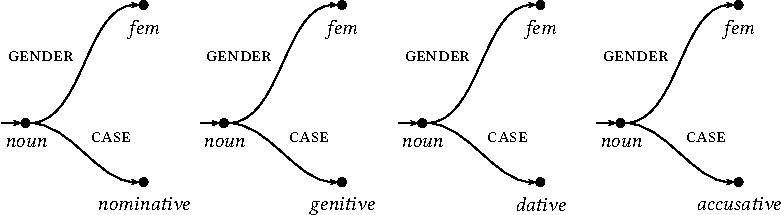
\includegraphics{Figures/frau-model-theoretic-cropped}
}
% \oneline{%
% \begin{pspicture}(-0.5,0.4)(2.8,4.1)
% %\psgrid


%      \psset{fillstyle=solid, fillcolor=black,radius=0.75mm}
%      \pnode(-0.4,2){start1}
%      \Cnode(0,2){noun1}
%      \Cnode(2,4){fem1}
%      \Cnode(2,1){nom1}


%      \psset{fillstyle=none,nodesep=0pt,angleB=180,arrows=->} 

%      \nccurve{start1}{noun1}
%      \nccurve{noun1}{fem1}\naput{\textsc{genus}}
%      \nccurve{noun1}{nom1}\naput{\textsc{kasus}}

%      \nput{270}{noun1}{\type{noun}}
%      \nput{270}{fem1}{\type{fem}}
%      \nput{270}{nom1}{\type{Nominativ}}
% \end{pspicture}
% \begin{pspicture}(-0.5,0.4)(2.8,4.1)
% %\psgrid


%      \psset{fillstyle=solid, fillcolor=black,radius=0.75mm}
%      \pnode(-0.4,2){start2}
%      \Cnode(0,2){noun2}
%      \Cnode(2,4){fem2}
%      \Cnode(2,1){nom2}


%      \psset{fillstyle=none,nodesep=0pt,angleB=180,arrows=->} 

%      \nccurve{start2}{noun2}
%      \nccurve{noun2}{fem2}\naput{\textsc{genus}}
%      \nccurve{noun2}{nom2}\naput{\textsc{kasus}}

%      \nput{270}{noun2}{\type{noun}}
%      \nput{270}{fem2}{\type{fem}}
%      \nput{270}{nom2}{\type{Genitiv}}
% \end{pspicture}
% \begin{pspicture}(-0.5,0.4)(2.8,4.1)
% %\psgrid


%      \psset{fillstyle=solid, fillcolor=black,radius=0.75mm}
%      \pnode(-0.4,2){start2}
%      \Cnode(0,2){noun2}
%      \Cnode(2,4){fem2}
%      \Cnode(2,1){nom2}


%      \psset{fillstyle=none,nodesep=0pt,angleB=180,arrows=->} 

%      \nccurve{start2}{noun2}
%      \nccurve{noun2}{fem2}\naput{\textsc{genus}}
%      \nccurve{noun2}{nom2}\naput{\textsc{kasus}}

%      \nput{270}{noun2}{\type{noun}}
%      \nput{270}{fem2}{\type{fem}}
%      \nput{270}{nom2}{\type{Dativ}}
% \end{pspicture}
% \begin{pspicture}(-0.5,0.4)(2.8,4.1)
% %\psgrid


%      \psset{fillstyle=solid, fillcolor=black,radius=0.75mm}
%      \pnode(-0.4,2){start2}
%      \Cnode(0,2){noun2}
%      \Cnode(2,4){fem2}
%      \Cnode(2,1){nom2}


%      \psset{fillstyle=none,nodesep=0pt,angleB=180,arrows=->} 

%      \nccurve{start2}{noun2}
%      \nccurve{noun2}{fem2}\naput{\textsc{genus}}
%      \nccurve{noun2}{nom2}\naput{\textsc{kasus}}

%      \nput{270}{noun2}{\type{noun}}
%      \nput{270}{fem2}{\type{fem}}
%      \nput{270}{nom2}{\type{Akkusativ}}
% \end{pspicture}}
\caption{\label{abb-avm-frau}Merkmalstrukturen zur Beschreibung von \emph{Frau} in (\ref{avm-frau})}
\end{figure}
%-----------------------------------------------------------------------------
\begin{figure}
%\oneline{%
\centerline{%
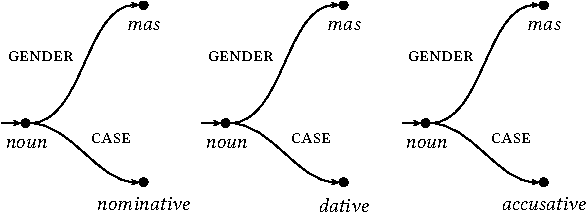
\includegraphics{Figures/mann-model-theoretic-cropped}
}
% \begin{pspicture}(-0.5,0.4)(2.8,4.1)
% %\psgrid
% %
% %
%      \psset{fillstyle=solid, fillcolor=black,radius=0.75mm}
%      \pnode(-0.4,2){start1}
%      \Cnode(0,2){noun1}
%      \Cnode(2,4){mas1}
%      \Cnode(2,1){nom1}
% %
% %
%      \psset{fillstyle=none,nodesep=0pt,angleB=180,arrows=->} 
% %
%      \nccurve{start1}{noun1}
%      \nccurve{noun1}{mas1}\naput{\textsc{genus}}
%      \nccurve{noun1}{nom1}\naput{\textsc{kasus}}
% %
%      \nput{270}{noun1}{\type{noun}}
%      \nput{270}{mas1}{\type{mas}}
%      \nput{270}{nom1}{\type{Nominativ}}
% \end{pspicture}
% \begin{pspicture}(-0.5,0.4)(2.8,4.1)
% %\psgrid
% %
%      \psset{fillstyle=solid, fillcolor=black,radius=0.75mm}
%      \pnode(-0.4,2){start2}
%      \Cnode(0,2){noun2}
%      \Cnode(2,4){mas2}
%      \Cnode(2,1){nom2}
% %
% %
%      \psset{fillstyle=none,nodesep=0pt,angleB=180,arrows=->} 
% %
%      \nccurve{start2}{noun2}
%      \nccurve{noun2}{mas2}\naput{\textsc{genus}}
%      \nccurve{noun2}{nom2}\naput{\textsc{kasus}}
% %
%      \nput{270}{noun2}{\type{noun}}
%      \nput{270}{mas2}{\type{mas}}
%      \nput{270}{nom2}{\type{Dativ}}
% \end{pspicture}
% \begin{pspicture}(-0.5,0.4)(2.8,4.1)
% %\psgrid
% %
%      \psset{fillstyle=solid, fillcolor=black,radius=0.75mm}
%      \pnode(-0.4,2){start2}
%      \Cnode(0,2){noun2}
%      \Cnode(2,4){mas2}
%      \Cnode(2,1){nom2}
% %
% %
%      \psset{fillstyle=none,nodesep=0pt,angleB=180,arrows=->} 
% %
%      \nccurve{start2}{noun2}
%      \nccurve{noun2}{mas2}\naput{\textsc{genus}}
%      \nccurve{noun2}{nom2}\naput{\textsc{kasus}}
% %
%      \nput{270}{noun2}{\type{noun}}
%      \nput{270}{mas2}{\type{mas}}
%      \nput{270}{nom2}{\type{Akkusativ}}
% \end{pspicture}}
\caption{\label{abb-avm-mann}Merkmalstrukturen zur Beschreibung von \emph{Mann} in  (\ref{avm-mann})}
\end{figure}
In diesen Darstellungen gehört zu jedem Knoten ein Typ (\type{noun}, \type{fem}, \type{Nominativ},
\ldots), wobei die Typen in den Merkmalstrukturen immer maximal spezifisch sind, \dash keine
Untertypen mehr haben. Es gibt immer einen Eingangsknoten (im Beispiel \type{noun}), und die anderen
Knoten sind mit Pfeilen verbunden, an denen jeweils die Merkmalsnamen (\textsc{genus}, \textsc{kasus}) stehen.

Geht man noch einmal zum Personenbeispiel aus den vorigen Abschnitten zurück,
so kann man sich den Unterschied zwischen Modell und Beschreibung so verdeutlichen:
%\NOTE{JB: unklar, Vor allem der Begriff M-Beschreibung/beschreibt ist ihm nicht klar}
Wenn wir ein Modell von Personen haben, das Vorname, Nachname, Geburtstag,
Geschlecht und Haarfarbe enthält, dann ist es klar, dass jedes modellierte Objekt
einen Geburtstag hat, wir können aber in Beschreibungen die Angaben in bezug
auf den Geburtstag weglassen, wenn diese bei der Formulierung von Beschränkungen
oder Suchen unwichtig sind.

Den Zusammenhang zwischen (linguistischen) Phänomenen, dem Modell
und der formalen Theorie verdeutlicht Abbildung~\vref{abb-modell}.
\begin{figure}[htbp]
\centerline{%
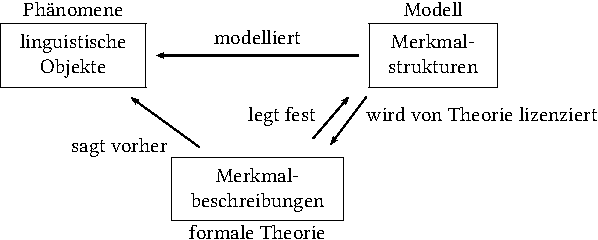
\includegraphics{Figures/model-theory-phenomenon-crop}
}
% %{
% \begin{pspicture}(0,0)(10.4,5)
% %\psgrid
% \rput[Bl](0,0){%
% \begin{tabular}[b]{@{}ccc@{}}
% Phänomen && Modell\\
% \rnode{phen}{\fbox{\begin{tabular}{c}
% Linguistische\\
% Objekte\\
% \end{tabular}}}&&\rnode{modell}{\fbox{\begin{tabular}{c}
% Merkmal-\\
% strukturen\\
% \end{tabular}}}\\[10ex]
% &\rnode{theorie}{\fbox{\begin{tabular}{c}
% Merkmal-\\
% beschreibungen\\
% \end{tabular}}}\\
% &Formale Theorie\\
% \end{tabular}}
% %\ncline{->}[l]{modell}[r]{phen}%
% \ncline{->}{modell}{phen}\nbput{modelliert}
% %\ncdiag[angleA=180,angleB=45]{->}{modell}{theorie}
% \psline{<-}(6.0,1.6)(6.6,2.6)
% \rput[Bl](6.6,2){wird von Theorie lizenziert} % früher Erfüllung, jetzt FR Änderung
% \psline{->}(5.175,1.7)(6.1,3.15)
% \rput[Bl](4.2,2.4){legt fest}
% %\nccurve{<-}{modell}{theorie}\nbput{legt fest}
% \ncline{->}{theorie}{phen}\naput{sagt vorher}%
% %\ncline{<->}[b]{modell}[tr]{theorie}%
% %\ncline{->}[tl]{theorie}[b]{phen}%
% \end{pspicture}
%\begin{pspicture}(0,0)(10.4,5)
%\psgrid
% \rput[Bl](0,0){%
% \begin{tabular}[b]{@{}ccc@{}}
% Phänomen && Modell\\
% \rnode{phen}{\fbox{\begin{tabular}{c}
% Linguistische\\
% Objekte\\
% \end{tabular}}}&&\rnode{modell}{\fbox{\begin{tabular}{c}
% Merkmal-\\
% strukturen\\
% \end{tabular}}}\\[10ex]
% &\rnode{theorie}{\fbox{\begin{tabular}{c}
% Merkmal-\\
% beschreibungen\\
% \end{tabular}}}\\
% &Formale Theorie\\
% \end{tabular}}
% %\anodeconnect[l]{modell}[r]{phen}%
% \ncline{->}{modell}{phen}\nbput{modelliert}
% %\ncdiag[angleA=180,angleB=45]{->}{modell}{theorie}
% \psline{<-}(6.0,1.6)(6.6,2.4)
% \rput[Bl](6.6,2){wird von Theorie lizenziert} % früher Erfüllung, jetzt FR Änderung
% \psline{->}(5.6,1.6)(6.2,2.4)
% \rput[Bl](4.5,2.4){legt fest}
% %\nccurve{<-}{modell}{theorie}\nbput{legt fest}
% \ncline{->}{theorie}{phen}\naput{sagt vorher}%
% %\aanodeconnect[b]{modell}[tr]{theorie}%
% %\anodeconnect[tl]{theorie}[b]{phen}%
% \end{pspicture}
\caption{\label{abb-modell}Phänomen, Modell und formale Theorie}
\end{figure}\nocite{Netter98a}%S. 26
%\NOTE{WS: zwischen Modell und Theorie sollten zwei Pfeile sein.}
% ###########
% zwei Pfeile: Beschreibung legt Modell fest , um Rekursion zu erfassen (beschreibt geht wohl auch, ist aber sloppy)
%
% Modell wird von der formalen Theorie lizenziert. 
%
% Phänomen + Modell -> PS: modelliert -> lassen wir so.
%
Das Modell modelliert linguistische Phänomene. Es muss außerdem
%alle Beschränkungen unserer Theorie erfüllen. 
von unserer Theorie lizenziert werden.
Die Theorie legt das Modell fest % FR: festlegen  gibt mehrere Modelle, exhaustive Modell enthält alle Sätze
und macht außerdem Vorhersagen in bezug auf mögliche
Phänomene.

In den folgenden Kapiteln wird eine Theorie des Deutschen entwickelt.
Das bedeutet, dass geklärt wird, welche Merkmale zur Modellierung
von Sprache benötigt werden und welche Werte diese Merkmale im Deutschen haben
können. Die Theorie formuliert Beschränkungen über das Auf"|treten
bestimmter Werte bzw.\ die Gleichheit von Werten.
\is{Modell|)}\is{Theorie|)}\is{Phänomen|)}\is{Merkmalbeschreibung|)}\is{Merkmalstruktur|)}
%}{}


\questions{

\begin{enumerate}
\item Weshalb verwendet man in der HPSG Typen?
\item Sind die folgenden Strukturen jeweils kompatibel, \dash, können sie benutzt werden,
      um dasselbe Objekt zu beschreiben?
\ea
\onems{
vorname  \type{max}\\
nachname \type{meier}\\
vater     \ms[person]{
              vorname  & peter\\
              nachname & meier\\
             }\\
}\hspace{0.5cm}\onems{
vorname  \type{max}\\
nachname \type{meier}\\
vater    \ms[person]{
              vorname  & peter\\
              nachname & müller\\
             }\\
}
\z
\ea
\onems{
vorname   \type{max}\\
nachname  \type{meier}\\
vater      \ms[person]{
              vorname  & peter\\
              nachname & meier\\
             }\\
}\hspace{0.5cm}\onems{
vorname   \type{max}\\
nachname  \type{meier}\\
mutter      \ms[person]{
              vorname  & ursula\\
              nachname & müller\\
             }\\
}
\z

\end{enumerate}
}


\exercises{

\begin{enumerate}
\item Überlegen Sie, wie man Musikinstrumente mittels Merkmalstrukturen beschreiben könnte.
\item\label{ua-liste} In diesem Kapitel wurden Listen eingeführt. Dies sieht wie eine Erweiterung des Formalismus
      aus. Dem ist aber nicht so, denn man kann die Listennotation in eine Notation überführen,
      die nur mit Merkmal"=Wert"=Paaren auskommt. Überlegen Sie, wie das geht.
\item (Zusatzaufgabe) Im folgenden Kapitel wird die Relation \emph{append}\is{Relation!\emph{append}} eine Rolle
      spielen, die dazu dient, zwei Listen zu einer dritten zu verknüpfen. Relationale
      Beschränkungen wie \emph{append} stellen eine Erweiterung des Formalismus dar. Mittels
      relationaler Beschränkungen kann man beliebige Werte von Merkmalen zu anderen Werten in
      Beziehung setzen, \dash, man kann kleine Programme schreiben, die einen Wert in Abhängigkeit von
      anderen Werten ausrechnen.  Es stellt sich die Frage, ob man solch mächtige Beschreibungsmittel in
      einer linguistischen Theorie braucht und wenn man sie zuläßt, was für eine Komplexität man
      ihnen zubilligt. Eine Theorie, die ohne relationale Beschränkungen auskommt, ist einer anderen
      vorzuziehen (siehe auch Kapitel~\ref{sec-kriterien} zum Vergleich von Theorien).

      Für die Verkettung von Listen gibt es eine direkte Umsetzung in Merkmalstrukturen ohne
      relationale Beschränkungen. Finden Sie diese. Geben Sie Ihre Quellen an und dokumentieren Sie,
      wie Sie bei der Suche nach der Lösung vorgegangen sind.
\end{enumerate}
}


\furtherreading{

Dieses Kapitel sollte den Leser auf leicht verständliche Weise an getypte Merkmalstrukturen heranführen.
Mathematische Eigenschaften der Strukturen, der Typhierarchien und der Verknüpfungsmöglichkeiten
solcher Strukturen können hier nicht erörtert werden. Die Kenntnis zumindest eines Teils dieser Eigenschaften
sind aber für die Arbeit in der Computerlinguistik und auch beim Entwickeln eigener Analysen
wichtig. Der interessierte Leser sei deshalb auf die folgenden Publikationen verwiesen:
%
Das Buch von \citet{Shieber86a} ist eine kurze Einführung in die Theorie der
Unifikationsgrammatiken. Es wird ein ziemlich allgemeiner Überblick gegeben, 
und wichtige Grammatik-Typen (DCG\is{Definite Clause Grammar@\textit{Definite Clause Grammar\/} (DCG)}, 
\lfg, \gpsg, HPSG, PATR-II\is{PATR-II}) werden vorgestellt.
%
\citet{Johnson88}
beschreibt den Formalismus ungetypter Merkmalstrukturen mathematisch exakt.
%
\citet{Carpenter92a} setzt sich sehr mathematisch mit getypten Merkmalstrukturen auseinander.  Der
Formalismus, den \citet{King99a-u} für HPSG"=Grammatiken entwickelt hat, bildet die Grundlage für
den von \citet{Richter2004a-u} entwickelten Formalismus, der derzeit als Standard gilt.

}

% FR: auch Pollard99 strong generative capacity. ist Variante auf Kings Modelltheorie

